\documentclass{article}
\usepackage[margin=1in]{geometry}
\usepackage{microtype}
\usepackage{setspace}
\usepackage{amsmath}
\usepackage{parskip}
\usepackage{amssymb}
\usepackage{graphicx}

\graphicspath{{../public/}}

\parskip=4ex
\date{}
\author{}

\title{12.1 Double Integrals Over Rectangles}

\begin{document}
  \maketitle
  \textbf{Introduction}\\
  In the same manner that integrating single variable functions, we obtained the area. We will be computing double integrals to find the volume of a solid.

  \textbf{Review of the Definite Integral}\\
  If $ f(x) $ is defined for $ a \le x\le b $, we start by dividing the interval $ [a,b] $ into $ n $ subintervals $ [x_{i-1},x_{i} ] $ with length $ \Delta x_{i}=x_{i}-x_{i-1} $ and choosing sample points $ x_{i}^{*} $ in these subintervals, visualized by the figure below.
  \begin{center}
    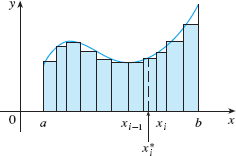
\includegraphics[width=6cm]{12_1_1}
  \end{center}

  The Riemann Sum equation form is obtained
  \[
   \sum^{n}_{i=1} f(x_{i}^{*}) \Delta x_{i} 
  \]
  Then by taking the limit of such sums as the hugest of the lengths approach 0 to obtain the definite integral of $ f $ from $ a \to b $
  \[
    \int^{b}_{a} f(x)~dx=\lim_{\text{max}\Delta x_{i} \to 0} \sum^{n}_{i=1} f(x_{i}^{*})\Delta x_{i}
  \]

  In the special case where $ f(x) \ge 0$, the Riemann sum can be intepreted as the sum of the areas of the approximating rectangles. Meaning that $ \int^{b}_{a} f(x)~dx $ represents the area under the curve $ y=f(x) $ from $ a\to b $. 

  \textbf{Volumes and Double Integrals}\\
  Then in a similar manner, a function $ f $ of two variables defined on a closed rectangle
  \[
    R=[a,b] \times [c,d] = \{ (x,y) \in \mathbb{R}^{2} | a \le x \le b,c \le y \le d \}
  \]
  And by suppousing that $ f(x,y) \ge 0 $. The graph of $ f $ is a surface with equation $ z=f(x,y) $. Let $ S $ be the solid that lies above $ R $ and  under the graph of $ f $ and under the graph of $ f $, that is
  \[
    S=\{ (x,y,z) \in \mathbb{R}^{2} | 0 \le z \le f(x,y), (x,y) \in \mathbb{R} \}
  \]
  
  Where our goal is to find the volume of $ S $
  \begin{center}
    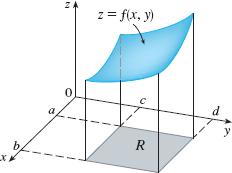
\includegraphics[width=6cm]{12_1_2}
  \end{center}

  To do so, we must take a partition $ P $ of $ R $ into sub rectangles. Done by dividing the intervals $ [a,b] ~\&~ [c,d] $.
  \[
    \begin{gathered}
    a = x_0 < x_1 < ... < x_{i-1} < x_i < x_{m} = b
    c = y_0 < y_1 < ... < y_{i-1} < y_i < y_{n} = d
    \end{gathered}
  \]

  By drawing lines parallel to the coordinate axes through these partition points like the figure below

  We form the subrectangles
  \[
    R_{ij}= [x_{i-1},x_i] \times [y_{j-1},y_j] = \{ (x,y) | x_{i-1} \le x \le x_{i}, y_{j-1} \le y \le y_j \}
  \]
  for $ i=1,...,m ~\&~ j=1,...,n$. There are $ mn $ of these subrectangles and they cover $ R $. By letting $ \Delta x_i = x_i - x_{i-1} ~\&~ \Delta y_j = y_j - y_{j-1}$, then we obtain the equation for the area of $ R_{ij} $
  \[
    \Delta A_{ij}= \Delta x_{i} \Delta y_{j}
  \]

  \begin{center}
    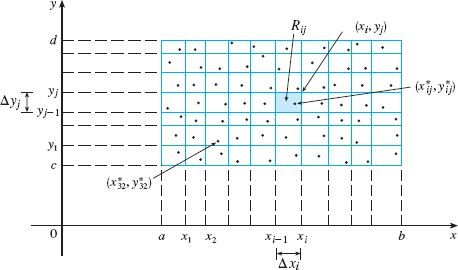
\includegraphics[width=10cm]{12_1_3}
  \end{center}

  By choosing a sample point $ (x^{*}_{ij}, y^{*}_{ij}) $ in each $ R_{ij} $, then we can approximate the part of $ S $ that lies above each $ R_{ij} $ by a thin column or rectangular box. This column has base $ R_{ij} ~\&~ $ height $ f(x^{*}_{ij}, y^{*}_{ij}) $ as shown below.  

  \begin{center}
    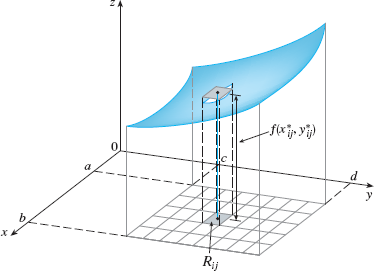
\includegraphics[width=10cm]{12_1_4}
  \end{center}

  The volume of this box is the height of the box times the area of the base rectangle.
  \[
    f(x^{*}_{ij},y^{*}_{ij}) \Delta A_{ij}
  \]

  By following this procedure for all the rectangles and summing up the volumes of the corresponding boxes, we get an approximation to the total volume of $ S $
  \[
    V \approx \sum^{m}_{i=1} \sum^{n}_{j=1} f(x^{*}_{ij},y^{*}_{ij}) \Delta A_{ij}
  \]
  
  The intuition behind this double Riemann sum means that for each subrectangle we evaluate $ f $ at the chosen point and multiply by the area of the subtectangle and summing up the results. Visualized by the figure below
  \begin{center}
    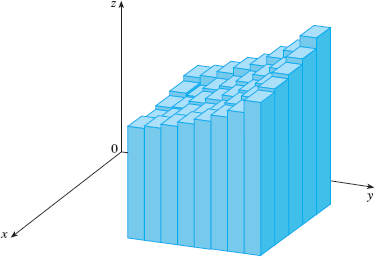
\includegraphics[width=10cm]{12_1_5}
  \end{center}

  The smaller the subrectangles become, the better the approximation becomes so we can take the limit of the Riemann sum to obtain
  \[
    V = \lim_{\text{max}\Delta x_i, \Delta y_j \to 0}  \sum^{m}_{i=1} \sum^{n}_{j=1} f(x^{*}_{ij},y^{*}_{ij}) \Delta A_{ij}
  \]
 
  \textbf{Def}\\
  The double integral of $ f $ over the rectangle $ R $ is
  \[
    \iint_R f(x,y)~ dA = \lim_{\text{max}\Delta x_i, \Delta y_j \to 0}  \sum^{m}_{i=1} \sum^{n}_{j=1} f(x^{*}_{ij},y^{*}_{ij}) \Delta A_{ij}
  \]

  if this limit exists.

  Now if $ f $ is integrable over $ R $, then the partitions $ P $ are regular, having the same dimensions and therefor the same area, $ \delta A = \Delta x \Delta y $. In this case by letting $ m\to \infty ~\&~ y\to \infty $. The sample point $ x^{*}_{ij},y^{*}_{ij} $ can be any point. However for simplicity sake, the sample point will be the upper right-hand corner of $ R_{ij} $, namely $ (x_i,y_j) $.
  \[
    \iint_R f(x,y)~dA = \lim_{m,n \to 0}  \sum^{m}_{i=1} \sum^{n}_{j=1} f(x^{*}_{i},y^{*}_{j}) \Delta A_{}
  \]
  
 By definition, the volume of our solid can be written as a double integral. 

 If $ f(x,y) \le 0$, then the volume $ V $ of the solid that lies above the rectangle $ R $ and below the surface $ z=f(x,y) $ is given by the equation
 \[
   V = \iint_R f(x,y)~dA
 \]

 \textbf{Ex 1}\\
 Estimate the volume of the solid that lies above the square $ R = [0,2] \ times [0,2] $ and below the elliptic paraboloid $ z=16-x^{2}-2y^{2} $. Divide $ R $ into four equal squares and choose the sample point to be the upper right corner of each square $ R_{ij} $.
 \[
   \begin{gathered}
   V \approx \sum^{2}_{i=1}\sum^{2}_{j=1} f(x_i,y_i) \Delta A\\
   f(1,1) \Delta A + f(1,2) \Delta + f(2,1) \Delta A + f(2,2) \Delta A\\
   13(1)+7(1)+10(1)+4(1) = \boxed{34}
   \end{gathered}
 \]

 \begin{center}
   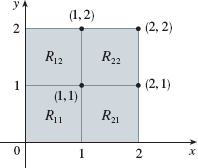
\includegraphics[width=6cm]{12_1_6} \qquad 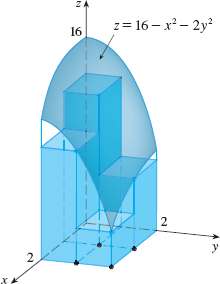
\includegraphics[width=4cm]{12_1_7}
 \end{center}

 \textbf{Ex 2}\\
 If $ R = \{ (x,y)|-1\le x\le1, -2 \le y \le 2 \} $, evaluate the integral $ \iint_{R}\sqrt{1-x^{2}} ~dA $ 
 \[
   \begin{gathered}
   \iint_R \sqrt{1-x^{2}} ~dA \to \int^{2}_{-2} \int^{1}_{-1}\sqrt{1-x^{2}} ~dydx\\
   ~\\
   \int^{2}_{-2} \text{\huge{[}} \int^{1}_{-1} \sqrt{1-x^{2}} ~dx \text{\huge{]}}dy \to \int^{2}_{-2} \text{\huge{]}} \int^{1}_{-1} \sqrt{1-\sin^{2}{\theta}} \cos{\theta}~d\theta \text{\huge{]}}dy\\
   x \to \frac{1}{1}\sin{\theta},~dx \to \cos{\theta}\\
   ~\\
   \int^{2}_{-2} \text{\huge{[}} \int^{1}_{-1} \sqrt{\cos^{2}{\theta}} \cos{\theta}~d\theta \text{\huge{]}}dy\\
   \int^{2}_{-2} \text{\huge{[}} \int^{1}_{-1} \cos^{2}{\theta}~d\theta \text{\huge{]}}dy\\
   \int^{2}_{-2} \text{\huge{[}} \int^{1}_{-1} \frac{\theta}{2}+\frac{\sin{2\theta}}{2} ~d\theta] \text{\huge{]}}dy\\
   x=\sin{\theta} \to \sin^{-1}{x} = \theta, \sin^{-1}{(1)} = \frac{\pi}{2}, \sin^{-1}{(-1)}=-\frac{\pi}{2}, ~ \theta = \pm \frac{\pi}{2}\\
   ~\\
   \int^{2}_{-2} \text{\huge{[}} \frac{\pi}{2} + \frac{\sin{2\theta}}{2} \text{\huge{]}}^{\theta=\frac{\pi}{2}}_{\theta=-\frac{\pi}{2}} ~dy = \int^{2}_{-2} \frac{\pi}{2}~dy = \frac{\pi}{2}y \bigg|^{y=2}_{y=-2}= \boxed{2\pi}
   \end{gathered}
 \]

 \textbf{The Midpoint Rule}
 \[
   \iint_R f(x,y)~dA \approx \sum^{m}_{i=1} \sum^{n}_{j=1} f(\overline{x}_i,\overline{y}_j) \Delta A 
 \]

 Where $ \overline{x}_i $ is the midpoint of $ [x_{i-1}, x_{i}] $ and $ \overline{y}_j $ is the midpoint of $ [y_{j-1}, y_j] $

 \textbf{Ex 3}\\
 Use the midpoint rule with $ m=n=2 $ to estimate the value of $ \iint_R (x-3y^{2})~dA $, where $ R= \{ (x,y) | 0 \le x \le 2, 1 \le y \le 2 \} $.
 \[
   \begin{gathered}
     \overline{x}_1 = \frac{1}{2}, \overline{x}_2 = \frac{3}{2}, \overline{y}_1 = \frac{5}{4}, \overline{y}_2 = \frac{7}{4}\\
     ~\\
     \Delta A = \frac{1}{2}\\
     ~\\
     \iint_R (x-3y^{2})~dA \approx \sum^{2}_{i=1} \sum^{2}_{j=1} f(\overline{x}_i, \overline{y}_j) \Delta A\\
     f(\overline{x}_1, \overline{y}_1) \Delta A + f(\overline{x}_2, \overline{y}_1) \Delta A + f(\overline{x}_1, \overline{y}_2) \Delta A + f(\overline{x}_2, \overline{y}_2) \Delta A = -\frac{95}{8} = \boxed{-11.875}
   \end{gathered}
 \]

 \begin{center}
   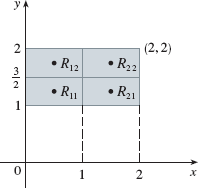
\includegraphics[width=6cm]{12_1_8}
 \end{center}

 \textbf{Iterated Integrals}
 \[
   \int^{b}_{a} \int^{d}_{c} f(x,y) ~dydx = \int^{b}_{a} \text{\huge{[}} \int^{d}_{c} f(x,y)~dy \text{\huge{]}}dx  
 \]

 Meaning that we first integrate with respect to $ y $ from $ c \to d $ and then integrate once again but this time with respect to x and from $ a \to b $.

 The inverse also follows like so
 \[
  \int^{d}_{c} \int^{b}_{a} f(x,y) ~dxdy = \int^{d}_{c} \text{\huge{[}} \int^{b}_{a} f(x,y)~dx \text{\huge{]}}dy 
 \]

 \textbf{Ex 4}\\
 Evaluate the following iterate integrals

 A) $ \int^{3}_{0} \int^{2}_{1} x^{2}y ~dydx$ 
 \[
   \begin{gathered}
     \int^{3}_{0} \int^{2}_{1} x^{2}y ~dydx \to \int^{3}_{0} \text{\huge{[}} \int^{2}_{1} x^{2}y~dydx \text{\huge{]}} ~dx\\
     \int^{3}_{0} x^{2}\frac{y^{2}}{2} \bigg|^{2}_{1}~dx \to \int^{3}_{0} \frac{3}{2}x^{2}~dx \to \frac{x^{3}}{2} \bigg|^{3}_0 \to \boxed{\frac{27}{2}}
   \end{gathered}
 \]
 
 B) $ \int^{2}_{1} \int^{3}_{0} x^{2}y ~ dxdy $
 \[
   \begin{gathered}
   \int^{2}_{1} \int^{3}_{0} dx~dy \to \int^{2}_{1} \text{\huge{[}} \int^{3}_{0} x^{2}y~dx \text{\huge{]}} ~dy\\
   \int^{2}_{1} \frac{x^{3}}{3}y^{2} \bigg|^{3}_0~dy \to \int^{2}_{1} 9y~dy \to 9y \bigg|^{2}_1 \to \boxed{\frac{27}{2}}
   \end{gathered}
 \]

 \textbf{Fubini's Theorem}\\
 If $ f $ is continuous on the rectangle $ R= \{ (x,y) | a \le x \le b, c \le y \le d \} $, then
 \[
   \iint_R f(x,y)~dA = \int^{b}_{a} \int^{d}_{c} f(x,y) ~dydx = \int^{d}_{c} \int^{b}_{a}f(x,y) ~ dxdy
 \]

 \textbf{Ex 6}\\
 Evaluate $ \iint_R y\sin{(xy)}~dA $, where $ R = [1,2] \times [0,\pi] $.
 \[
   \begin{gathered}
   \iint_R y\sin{(xy)}~dA \to \int^{\pi}_{0} \int^{2}_{1} y\sin{(xy)} ~dxdy = \int^{\pi}_{0} \text{\huge{[}} -\cos{(xy)} \text{\huge{]}}^{2}_1~dy\\
   \int^{\pi}_{0} (-\cos{(2y)}+\cos{y})~dy = -\frac{1}{2} \sin{(2y)}+\sin{y} \bigg|^{\pi}_0
   \end{gathered}
 \]

 Note that we can integrate in any order as the same answer will always be produced, however the order of integration also determines the difficulty of the integral as well.
 \[
   \iint_R y\sin{(xy)}~dA \to \int^{2}_{1} \int^{\pi}_{0} y\sin{(xy)} ~dydx
 \]
 
 If we were to integrate with respect to $ y $ first, the integral becomes much harder as it involves integration by parts twice. Therefore, we should integrate in whichever order is easiest.

 There are special cases where $ f(x,y) $ can be factored as the product of a function of $ x $ only and a function of $ y $ only. The double integral of $ f $ can be written in a simplier form. To exemplify, suppouse that $ f(x,y) = g(x) h(y) $ and $ R = [a,b] \times [c,d] $. Fubini's Theorem gives 

 \[
   \begin{gathered}
   \iint_R f(x,y)~dA \to \int^{d}_{c} \int^{b}_{a} g(x)h(y)~dxdy = \int^{d}_{c} \text{\huge{[}} \int^{b}_{a} g(x)h(y) ~dx \text{\huge{]}} dy 
   \end{gathered}
 \]

 In the inner integral $ y $ is a constant, so $ h(y) $ is a constant, allowing the equation to be written as so
 \[
   \begin{gathered}
   \int^{d}_{c} \text{\huge{[}} \int^{b}_{a} g(x)h(y)~dxdy = \int^{d}_{c} \text{\huge{[}} h(y)\int^{b}_{a} g(x)~dx \text{\huge{]}} dy =  \int^{b}_{a} g(x)~dx \int^{d}_{c} h(y) ~ dy 
   \end{gathered}
 \]

 Since $ \int^{b}_{a} g(x)~dx $ is a constant, so the double integral of $ f $ can be written as the product of two single integrals. 

 \textbf{Ex 8}\\
  Evaluate $ \iint_R \sin{x}\cos{y}~dA $, where $ R= [0,\frac{\pi}{2}] \times [0,\frac{\pi}{2}] $
  \[
    \begin{gathered}
    \iint_R \sin{x}\cos{y}~dA = \int^{\frac{\pi}{2}}_{0} \sin{x}~dx \int^{\frac{\pi}{2}}_{0} \cos{y}~dy\\
    -\cos{x}\bigg|^{\frac{\pi}{2}}_0 \cdot \sin{y}\bigg|^{\frac{\pi}{2}}_0 = 1 \cdot 1 = \boxed{1}
    \end{gathered}
  \]

  \textbf{Properties of Double Integrals}
  \[
    \iint_R f(x,y) + g(x,y)~dA = \iint_R f(x,y)~dA + \iint g(x,y)~dA
  \]
  \[
    \iint_R c f(x,y)~dA = c\iint_R f(x,y)~dA \qquad \text{where $ c $ is a constant}
  \]
\end{document}
